% !TeX program = xelatex
% AI for Theological Inquiry — Lecture 4 deck. Build: xelatex lecture04.tex (twice).
% beamer-slides house preamble.
% Copy into a new deck and edit \deckauthor / \deckemail / \deckdate / colors.
% Build: xelatex deck.tex (run twice). See ../SKILL.md for the full house style.
\documentclass[aspectratio=169,11pt]{beamer}

\usetheme{metropolis}
\usepackage{fontspec}
\usepackage{graphicx}
\usepackage{tikz}
\usetikzlibrary{arrows.meta,positioning,shapes.geometric,fit,shadows}
\usepackage{tcolorbox}
\tcbuselibrary{skins,breakable}
\usepackage{fontawesome5}
\usepackage{listings}
\usepackage{booktabs}
\usepackage{array}

% ---------------------------------------------------------------- palette
% Placeholder professional navy/accent palette — swap for the exact ANL/ALCF
% brand hex values if you have the brand guide; do not present these as
% "official" institutional colors.
\definecolor{labnavy}{RGB}{18,42,73}
\definecolor{labink}{RGB}{40,44,52}
\definecolor{accentgold}{RGB}{223,161,54}
\definecolor{accentteal}{RGB}{0,137,123}
\definecolor{accentblue}{RGB}{41,98,168}
\definecolor{lightgray}{RGB}{245,246,248}
\definecolor{midgray}{RGB}{110,118,129}

% Hard rule: background is always white.
\setbeamercolor{background canvas}{bg=white}
\setbeamercolor{palette primary}{bg=labnavy,fg=white}
\setbeamercolor{frametitle}{bg=labnavy,fg=white}
\setbeamercolor{progress bar}{fg=accentteal,bg=lightgray}
\setbeamercolor{normal text}{fg=labink}
\setbeamercolor{alerted text}{fg=accentgold}
\setbeamercolor{footline}{fg=midgray}
\setbeamerfont{footline}{size=\tiny}

% Tighter default itemize indentation (see SKILL.md Gotchas — do NOT pass
% [leftmargin=...] to Beamer's itemize, that slot is for overlay specs).
\setlength{\leftmargini}{14pt}

% ---------------------------------------------------------------- deck metadata
% Fill these in per-deck. Email + date are a hard rule on the title page.
\newcommand{\deckauthor}{Huihuo Zheng}
\newcommand{\deckemail}{huihuo.zheng@wheaton.edu}
\newcommand{\deckinstitute}{Wheaton College}
% \date{...} still needs to be called explicitly in the document, e.g. \date{\today}

% ---------------------------------------------------------------- logo
% Looks for a real logo file first; falls back to a plain text lockup rather
% than fabricating the institutional mark. Put the real file at
% logos/argonne_logo.pdf (or .png) next to the deck, or point this at a
% shared assets/logos/ path.
% Drop a real logo at logos/wheaton_logo.pdf (or .png) to use it; otherwise
% this falls back to a plain text lockup rather than fabricating the mark.
\newcommand{\decklogo}[1][0.16\textwidth]{%
  \IfFileExists{logos/wheaton_logo.pdf}%
    {
\includegraphics[width=#1]{logos/wheaton_logo.pdf}}%
    {\IfFileExists{logos/wheaton_logo.png}%
      {
\includegraphics[width=#1]{logos/wheaton_logo.png}}%
      {\begin{minipage}{#1}\centering
         {\Large\bfseries\textsc{\textcolor{labnavy}{Wheaton}}}\\[1pt]
         {\small\bfseries\textsc{\textcolor{labnavy}{College}}}
       \end{minipage}}}%
}

% Small corner logo on every content slide (title page uses \decklogo directly
% instead, usually larger — see templates/titlepage.tex). Comment out this
% \logo{} line if you don't want the small footer/corner logo repeated.
% Teaching deck: no repeated corner logo (title page carries it once).
% \logo{\IfFileExists{logos/argonne_logo.pdf}%
%   {\includegraphics[height=0.45cm]{logos/argonne_logo.pdf}}%
%   {\IfFileExists{logos/argonne_logo.png}%
%     {\includegraphics[height=0.45cm]{logos/argonne_logo.png}}{}}}

% ---------------------------------------------------------------- shadowed boxes
% House rule: every box gets a shadow. Pick "drop shadow" (crisp) or
% "drop fuzzy shadow" (soft) and use it consistently through one deck.
% IMPORTANT: "enhanced" is required for the shadow to render at all — without
% it tcolorbox silently accepts the "drop shadow"/"drop fuzzy shadow" key and
% draws nothing (no error, no warning). See SKILL.md Gotchas.
\newtcolorbox{featbox}[2]{
  enhanced,
  colback=lightgray, colframe=#1, boxrule=0.6pt, arc=3pt,
  left=6pt, right=6pt, top=4pt, bottom=4pt,
  title=#2, colbacktitle=#1, coltitle=white,
  fonttitle=\bfseries\small, boxsep=1pt,
  drop fuzzy shadow
}

\newtcolorbox{calloutbox}[1][labnavy]{
  enhanced,
  colback=#1!6, colframe=#1, boxrule=0.6pt, arc=3pt,
  left=10pt, right=10pt, top=6pt, bottom=6pt,
  drop fuzzy shadow
}

\lstdefinestyle{shell}{
  basicstyle=\ttfamily\scriptsize\color{labink},
  keywordstyle=\color{accentblue}\bfseries,
  commentstyle=\color{midgray}\itshape,
  stringstyle=\color{accentteal},
  backgroundcolor=\color{lightgray},
  frame=single, framerule=0.4pt, rulecolor=\color{midgray!60},
  breaklines=true, columns=fullflexible,
  xleftmargin=4pt, xrightmargin=4pt, framexleftmargin=4pt
}


% ---- palette aliases for this deck's three pillars (match lecture01/02/03) ----
\definecolor{cAgent}{RGB}{41,98,168}   % agentic AI  (blue)
\definecolor{cRAG}{RGB}{0,137,123}     % RAG         (teal)
\definecolor{cEval}{RGB}{223,161,54}   % evaluation  (gold)

\title{AI for Theological Inquiry}
\subtitle{Lecture 4 --- Sources \& the theological corpus: \emph{what} you ground on}
\date{September 22, 2026}

\begin{document}

% beamer-slides house title page.
% Requires preamble.tex to be loaded first (\decklogo, \deckauthor, \deckemail,
% \deckinstitute). Set \title{}/\subtitle{} and \date{} before this frame.
%
% Hard rule: title page always shows author name, email, and date. Email sits
% bottom-left in small type, footnote-style — not in the author block.

\begin{frame}[plain]
  \begin{columns}[c]
    \begin{column}{0.32\textwidth}
      \centering
      \decklogo[0.9\textwidth]
    \end{column}
    \begin{column}{0.66\textwidth}
      {\usebeamerfont{title}\usebeamercolor[fg]{title}\Huge\bfseries \inserttitle\par}
      \ifx\insertsubtitle\@empty\else
        \vspace{4pt}
        {\large\color{midgray}\insertsubtitle\par}
      \fi
      \vspace{18pt}
      {\small
        \deckauthor\\
        \deckinstitute\\
        \insertdate}
    \end{column}
  \end{columns}
  \vfill
  {\footnotesize\color{midgray}\deckemail\par}
\end{frame}


% ---------------------------------------------------------------- recap / where we are
\begin{frame}{Where we are: last week, \emph{why} grounding matters}
  \begin{columns}[c, totalwidth=\textwidth]
    \begin{column}{0.47\textwidth}
      \begin{featbox}{accentgold}{\faGhost\ Last week}
        \small
        \begin{itemize}
          \item Wrapped the agent loop back on the raw model
          \item Vibe-coded a tool --- and \textbf{baked a fabricated verse into code that ran green}
          \item The rule: \emph{ground it, prove it, disclose it}
        \end{itemize}
        {\scriptsize\color{midgray}You saw \emph{why} you must ground.}
      \end{featbox}
    \end{column}
    \begin{column}{0.06\textwidth}\end{column}
    \begin{column}{0.47\textwidth}
      \begin{featbox}{cRAG}{\faLayerGroup\ This week}
        \small
        \begin{itemize}
          \item Grounding means retrieving from \textbf{real sources}
          \item So: \textbf{which} sources? \textbf{whose} text?
          \item Assemble the \textbf{term corpus} --- the texts you ground on all term
        \end{itemize}
        {\scriptsize\color{midgray}You choose \emph{what} to ground \emph{on}.}
      \end{featbox}
    \end{column}
  \end{columns}
  \vspace{10pt}
  \begin{center}\small\color{labnavy}\bfseries
    First, though --- a proper look at the thing you actually did last week: \emph{vibe coding}.\end{center}
\end{frame}

% ================================================================================
% RECAP BLOCK — vibe coding, systematically (~15 min). Remove this block to
% restore the original 12-page Lecture 4; nothing downstream depends on it.
% ================================================================================

% ---------------------------------------------------------------- recap 1: the definition
\begin{frame}{Recap 1/5 --- ``Vibe coding'': what the term actually means}
  \begin{calloutbox}[accentgold]
    \small\faQuoteLeft\ \emph{``There's a new kind of coding I call `vibe coding', where you fully
    give in to the vibes, embrace exponentials, and \textbf{forget that the code even exists}
    \ldots\ I `Accept All' always, I don't read the diffs anymore.''}
    \hfill{\scriptsize\color{midgray}--- Andrej Karpathy, February 2025}
  \end{calloutbox}
  \vspace{6pt}
  \begin{columns}[t, totalwidth=\textwidth]
    \begin{column}{0.48\textwidth}
      \begin{featbox}{midgray}{\faIcon{exchange-alt}\ The term has already drifted}
        \scriptsize
        In everyday use ``vibe coding'' has come to mean \emph{any} AI-assisted coding.
        That is not what it named. The original sense is narrower --- and much sharper.
      \end{featbox}
    \end{column}
    \begin{column}{0.04\textwidth}\end{column}
    \begin{column}{0.48\textwidth}
      \begin{featbox}{accentgold}{\faEyeSlash\ The load-bearing word is \emph{not}}
        \scriptsize
        Not the model. Not the tool. Not the speed. \textbf{You do not read the code.}
        Everything else about vibe coding follows from that one omission.
      \end{featbox}
    \end{column}
  \end{columns}
  \vspace{4pt}
  \begin{center}\small\color{labnavy}\bfseries
    So the definition is not about what the machine did. It is about \emph{what you chose not to look at}.\end{center}
\end{frame}

% ---------------------------------------------------------------- recap 2: the loop
\begin{frame}{Recap 2/5 --- The loop, and where you sit in it}
  \begin{center}
  \begin{tikzpicture}[font=\scriptsize, node distance=0.5cm,
      s/.style={rectangle, rounded corners=3pt, draw, thick, fill=lightgray,
                drop shadow, align=center, text width=1.65cm, minimum height=0.9cm},
      h/.style={rectangle, rounded corners=2pt, draw=accentgold, very thick,
                fill=accentgold!15, align=center, font=\tiny\bfseries, inner sep=3pt}]
    \node[s, draw=labnavy]              (p) {\faKeyboard\\ \textbf{Prompt}};
    \node[s, draw=cAgent,  right=of p]  (g) {\faRobot\\ \textbf{Generate}\\ \scriptsize code};
    \node[s, draw=accentblue, right=of g] (r) {\faPlay\\ \textbf{Run}};
    \node[s, draw=cRAG,    right=of r]  (o) {\faEye\\ \textbf{Observe}\\ \scriptsize output / error};
    \node[s, draw=cEval,   right=of o]  (a) {\faCheckDouble\\ \textbf{Accept?}};
    \draw[-{Latex[length=5pt]}, thick, midgray] (p)--(g);
    \draw[-{Latex[length=5pt]}, thick, midgray] (g)--(r);
    \draw[-{Latex[length=5pt]}, thick, midgray] (r)--(o);
    \draw[-{Latex[length=5pt]}, thick, midgray] (o)--(a);
    \draw[-{Latex[length=5pt]}, thick, midgray] (o) to[out=-115,in=-65]
      node[below, font=\tiny, midgray, yshift=1pt] {the agent self-fixes --- often many times, unattended} (g);
    \node[h, above=0.3cm of p] {\faUser\ YOU};
    \node[h, above=0.3cm of a] {\faUser\ YOU};
  \end{tikzpicture}
  \end{center}
  \vspace{2pt}
  \begin{columns}[t, totalwidth=\textwidth]
    \begin{column}{0.48\textwidth}
      \begin{featbox}{accentgold}{\faUser\ You touch the loop exactly twice}
        \scriptsize
        You write the \textbf{prompt} and you make the \textbf{accept decision}.
        Everything between is the agent. Vibe coding is what happens when that
        second touch becomes automatic.
      \end{featbox}
    \end{column}
    \begin{column}{0.04\textwidth}\end{column}
    \begin{column}{0.48\textwidth}
      \begin{featbox}{cAgent}{\faIcon{sync-alt}\ Why the loop is the whole story}
        \scriptsize
        An LLM answers \emph{once}; an agent \textbf{runs the loop} until something looks
        done. ``Looks done'' is measured by the \emph{program running} --- never by the
        program being \emph{right}.
      \end{featbox}
    \end{column}
  \end{columns}
\end{frame}

% ---------------------------------------------------------------- recap 3: the dial
\begin{frame}{Recap 3/5 --- It is a dial, not a switch}
  \vspace{-2pt}
  \begin{center}
  \renewcommand{\arraystretch}{1.35}
  \begin{tabular}{@{}c>{\raggedright\arraybackslash}p{2.9cm}>{\raggedright\arraybackslash}p{3.9cm}>{\raggedright\arraybackslash}p{3.4cm}@{}}
    \toprule
    & \textbf{\scriptsize Level} & \textbf{\scriptsize What you actually read}
      & \textbf{\scriptsize Honest use} \\
    \midrule
    {\color{accentteal}\faCircle} & \scriptsize L0 $\cdot$ Autocomplete
      & \scriptsize Every line; you wrote it & \scriptsize Anything \\
    {\color{accentteal}\faCircle} & \scriptsize L1 $\cdot$ Assisted
      & \scriptsize Every generated line & \scriptsize Anything \\
    {\color{accentblue}\faCircle} & \scriptsize L2 $\cdot$ Delegated
      & \scriptsize The diff and the tests & \scriptsize Work you will defend \\
    {\color{accentgold}\faCircle} & \scriptsize L3 $\cdot$ \textbf{Vibe}
      & \scriptsize Only that it \emph{ran} & \scriptsize Prototypes only \\
    {\color{labnavy}\faCircle} & \scriptsize L4 $\cdot$ Autonomous
      & \scriptsize Nothing at all & \scriptsize \emph{Not research} \\
    \bottomrule
  \end{tabular}
  \end{center}
  \vspace{6pt}
  \begin{center}\small\color{labnavy}
    \faLightbulb\ Last week you ran at \textbf{L3} on purpose --- that is why the fabrication got
    through.\\[1pt]
    \textbf{No rung is a sin; landing on one by accident is.}
    Pick the rung before you prompt --- and name it when you disclose.
  \end{center}
\end{frame}

% ---------------------------------------------------------------- recap 4: failure taxonomy
\begin{frame}{Recap 4/5 --- Five ways vibes fail (one matters most here)}
  \begin{featbox}{accentgold}{\faGhost\ 1. Fabrication --- the one that bites \emph{this} course}
    \small
    Invented facts hard-coded \textbf{as data} --- last week's wrong Philemon 1:6,
    in a script that \textbf{ran green}.
  \end{featbox}
  \vspace{3pt}
  {\small
  \begin{itemize}\setlength{\itemsep}{2pt}
    \item \textbf{2. Plausible-but-wrong logic} --- it runs; the semantics are off.
          A stop-word list that drops \emph{``not''}.
    \item \textbf{3. Silent scope creep} --- it rewrote a file you never mentioned.
    \item \textbf{4. Dependency and licence debt} --- packages and provenance you did not choose.
    \item \textbf{5. Comprehension debt} --- you cannot debug, defend, or
          \textbf{disclose} what you never read.
  \end{itemize}}
  \vspace{4pt}
  \begin{center}\small\color{labnavy}\bfseries
    Code \emph{launders} a claim: in a chat window it looks like a guess ---
    in a script it looks like a \textbf{result}.\end{center}
\end{frame}

% ---------------------------------------------------------------- recap 5: the discipline + bridge
\begin{frame}{Recap 5/5 --- The discipline, and today's version of it}
  \begin{center}
    \begin{tcolorbox}[enhanced, width=0.82\textwidth, colback=labnavy!7, colframe=labnavy,
                      boxrule=0.9pt, arc=3pt, drop fuzzy shadow, halign=center,
                      top=5pt, bottom=5pt]
      {\large\bfseries\color{labnavy} Vibe to explore. Verify to publish.}
    \end{tcolorbox}
  \end{center}
  \vspace{2pt}
  \begin{columns}[t, totalwidth=\textwidth]
    \begin{column}{0.48\textwidth}
      \begin{featbox}{cAgent}{\faListOl\ Four moves that turn L3 into L2}
        \scriptsize
        \begin{enumerate}
          \item \textbf{Read} what it wrote --- at minimum the diff
          \item \textbf{Ground} every factual claim in a real source {\color{cRAG}(RAG --- Wk 4)}
          \item \textbf{Test} it against something you can check {\color{cEval}(Eval --- Wk 6)}
          \item \textbf{Disclose} model, tool, and \emph{which rung} you were on
        \end{enumerate}
      \end{featbox}
    \end{column}
    \begin{column}{0.04\textwidth}\end{column}
    \begin{column}{0.48\textwidth}
      \begin{featbox}{cRAG}{\faScroll\ The same rule in new clothes}
        \scriptsize
        In this afternoon's lab the agent will happily fetch and clean your texts ---
        fast, and worth using. But \emph{it} cannot tell you which canon, which
        translation, or which licence it just handed you.
        \vspace{3pt}
        \begin{center}\normalsize\bfseries\color{labnavy}
          Vibe to \emph{fetch}. Verify to \emph{keep}.\end{center}
      \end{featbox}
    \end{column}
  \end{columns}
  \vspace{6pt}
  \begin{center}\small\color{labnavy}\bfseries
    Next week we build the retriever. This week we decide what it is allowed to find.\end{center}
\end{frame}

% ================================================================================
% END RECAP BLOCK
% ================================================================================

% ---------------------------------------------------------------- the pipeline inherits
\begin{frame}{Everything downstream inherits what you choose here}
  \begin{center}
  
\begin{tikzpicture}[font=\scriptsize, node distance=0.55cm,
      s/.style={rectangle, rounded corners=3pt, draw, thick, fill=lightgray,
                drop shadow, align=center, text width=1.55cm, minimum height=0.9cm}]
    \node[s, draw=labnavy]     (src) {\faScroll\\ \textbf{Sources}\\ \scriptsize \emph{today}};
    \node[s, draw=cAgent, right=of src] (cl)  {\faBroom\\ \textbf{Clean}\\ \scriptsize + metadata};
    \node[s, draw=accentblue, right=of cl] (ch) {\faCut\\ \textbf{Chunk}\\ \scriptsize passages};
    \node[s, draw=cRAG, right=of ch] (em) {\faVectorSquare\\ \textbf{Embed}\\ \scriptsize vectors};
    \node[s, draw=cEval, right=of em] (rt) {\faComments\\ \textbf{Retrieve}\\ \scriptsize + cite};
    \draw[-{Latex[length=5pt]}, thick, midgray] (src)--(cl);
    \draw[-{Latex[length=5pt]}, thick, midgray] (cl)--(ch);
    \draw[-{Latex[length=5pt]}, thick, midgray] (ch)--(em);
    \draw[-{Latex[length=5pt]}, thick, midgray] (em)--(rt);
  \end{tikzpicture}
  \end{center}
  \vspace{4pt}
  \begin{columns}[t, totalwidth=\textwidth]
    \begin{column}{0.48\textwidth}
      \begin{featbox}{cRAG}{\faArrowLeft\ Garbage in $\to$ grounded in garbage}
        \scriptsize A perfect retriever over the \textbf{wrong edition} cites the wrong
        text --- \emph{confidently, with a page number}. The corpus is the ceiling on
        everything the agent can honestly say.
      \end{featbox}
    \end{column}
    \begin{column}{0.04\textwidth}\end{column}
    \begin{column}{0.48\textwidth}
      \begin{featbox}{accentblue}{\faExclamationCircle\ The data is not neutral}
        \scriptsize Which books, which translation, which manuscript, which notes ---
        each is a \textbf{decision} someone already made. You inherit it, so you must
        \textbf{see it}.
      \end{featbox}
    \end{column}
  \end{columns}
\end{frame}

% ---------------------------------------------------------------- where sources live
\begin{frame}{Where digital primary sources live (public-domain first)}
  \begin{columns}[t, totalwidth=\textwidth]
    \begin{column}{0.31\textwidth}
      \begin{featbox}{cAgent}{\faBookOpen\ Scripture (openly licensed)}
        \scriptsize \textbf{World English Bible} (public domain), \textbf{KJV}, ASV,
        Darby, Young's Literal --- via \texttt{bible-api.com}, STEP Bible, or plain text.
      \end{featbox}
    \end{column}
    \begin{column}{0.035\textwidth}\end{column}
    \begin{column}{0.31\textwidth}
      \begin{featbox}{cRAG}{\faLandmark\ Classics \& the Fathers}
        \scriptsize \textbf{CCEL} (ccel.org) --- Augustine, Aquinas, Calvin, Luther;
        \textbf{Project Gutenberg}; \textbf{Sacred-Texts} across traditions.
      \end{featbox}
    \end{column}
    \begin{column}{0.035\textwidth}\end{column}
    \begin{column}{0.31\textwidth}
      \begin{featbox}{cEval}{\faLanguage\ Originals \& critical text}
        \scriptsize \textbf{Perseus} (Greek/Latin), SBLGNT, open Hebrew (OSHB) ---
        when the \emph{original language} is the object of study.
      \end{featbox}
    \end{column}
  \end{columns}
  \vspace{10pt}
  \begin{calloutbox}[cRAG]
    \small\faInfoCircle\ \textbf{Prefer public-domain / open-licensed sources.} They are
    reproducible, redistributable, and \emph{disclosable} --- the same values that made
    us run on an open ALCF model. Modern copyrighted translations come with strings (next-but-one slide).
  \end{calloutbox}
\end{frame}

% ================================================================ the loaded data
\begin{frame}{The heart of today: ``the data is theologically loaded''}
  \begin{center}
  \begin{tikzpicture}[font=\scriptsize, node distance=0.45cm and 0.6cm,
      s/.style={rectangle, rounded corners=3pt, draw, thick, fill=lightgray,
                drop shadow, align=center, text width=3.2cm, minimum height=1.15cm}]
    \node[s, draw=labnavy]  (can) {\faBook\\ \textbf{Canon}\\ \scriptsize which books count?};
    \node[s, draw=cAgent, right=of can] (tra) {\faLanguage\\ \textbf{Translation}\\ \scriptsize whose words?};
    \node[s, draw=cRAG, below=of can] (txt) {\faScroll\\ \textbf{Text / manuscript}\\ \scriptsize which base text?};
    \node[s, draw=cEval, right=of txt] (par) {\faStickyNote\\ \textbf{Paratext}\\ \scriptsize whose headings \& notes?};
  \end{tikzpicture}
  \end{center}
  \vspace{4pt}
  \begin{center}\small\color{labnavy}\bfseries
    Four decisions are \emph{already made} inside any text file you download.\end{center}
  \vspace{2pt}
  \begin{center}\scriptsize\color{midgray}%
    None is a bug to ``fix.'' Each is a scholarly choice --- your job is to \textbf{name} it and \textbf{disclose} it.\end{center}
\end{frame}

% ---------------------------------------------------------------- canon + translation
\begin{frame}{Canon \& translation: the choice is theology, not plumbing}
  \begin{columns}[t, totalwidth=\textwidth]
    \begin{column}{0.48\textwidth}
      \begin{featbox}{labnavy}{\faBook\ Canon --- which books?}
        \scriptsize
        Protestant \textbf{66} $\cdot$ Catholic \textbf{73} (Tobit, Judith, Wisdom,
        Sirach, 1--2 Maccabees\dots) $\cdot$ Orthodox more.
        \\[3pt]\textbf{Download ``the Bible'' and you have quietly chosen a canon.}
      \end{featbox}
    \end{column}
    \begin{column}{0.04\textwidth}\end{column}
    \begin{column}{0.48\textwidth}
      \begin{featbox}{cAgent}{\faLanguage\ Translation --- whose words?}
        \scriptsize
        Isaiah 7:14: KJV/ESV \emph{``a \textbf{virgin} shall conceive''} vs NRSV
        \emph{``a \textbf{young woman}''} (Heb.\ \emph{almah}).
        \\[3pt]\textbf{Same verse, different doctrine implied --- by the translator.}
      \end{featbox}
    \end{column}
  \end{columns}
  \vspace{8pt}
  \begin{calloutbox}[accentgold]
    \small\faQuestionCircle\ Ask your RAG agent \emph{``what does the Bible say about X?''}
    --- and it answers from \textbf{the canon and translation you loaded}, with no idea
    it made a choice. \textbf{You} have to know which Bible is in the box.
  \end{calloutbox}
\end{frame}

% ---------------------------------------------------------------- text/manuscript + paratext
\begin{frame}{Text \& paratext: the words that may not be original}
  \begin{columns}[t, totalwidth=\textwidth]
    \begin{column}{0.48\textwidth}
      \begin{featbox}{cRAG}{\faScroll\ Manuscript / base text}
        \scriptsize
        \emph{Textus Receptus} (KJV) vs the \textbf{critical text} (NA28). Disputed
        passages: the \textbf{longer ending of Mark} (16:9--20), the \emph{pericope
        adulterae} (John 7:53--8:11), the \emph{Comma Johanneum} (1 John 5:7).
        \\[3pt]\textbf{Present, bracketed, or footnoted --- depending on your file.}
      \end{featbox}
    \end{column}
    \begin{column}{0.04\textwidth}\end{column}
    \begin{column}{0.48\textwidth}
      \begin{featbox}{cEval}{\faStickyNote\ Paratext --- the editor's hand}
        \scriptsize
        Chapter \& verse numbers (\textbf{medieval}, not original), section headings,
        cross-refs, study notes --- all \textbf{added}.
        \\[3pt]\textbf{Chunk by ``verse'' and you have adopted a 13th-c.\ editor's
        boundaries as your unit of meaning.}
      \end{featbox}
    \end{column}
  \end{columns}
  \vspace{8pt}
  \begin{center}\small\color{labnavy}\bfseries
    How you \emph{chunk} (next week) is itself interpretive --- verse, pericope, or paragraph?\end{center}
\end{frame}

% ---------------------------------------------------------------- copyright / licensing
\begin{frame}{Copyright: why we ground on public-domain translations}
  \begin{center}
  \begin{tikzpicture}[font=\scriptsize, node distance=0.7cm,
      d/.style={diamond, aspect=2, draw, thick, fill=lightgray, drop shadow, align=center, text width=2.2cm},
      s/.style={rectangle, rounded corners=3pt, draw, thick, fill=lightgray, drop shadow, align=center, text width=3.9cm, minimum height=0.8cm}]
    \node[d, draw=labnavy] (q) {Is it public\\ domain / open?};
    \node[s, draw=cRAG, right=2.2cm of q] (yes) {\faUnlock\ \textbf{WEB, KJV, ASV, Fathers}\\ \scriptsize embed, redistribute, cite freely};
    \node[s, draw=accentgold, below=0.45cm of yes] (no) {\faLock\ \textbf{NIV, ESV, NRSV}\\ \scriptsize copyrighted --- limited quoting, no bulk embedding};
    \draw[-{Latex[length=5pt]}, thick, cRAG] (q) -- node[above,font=\scriptsize]{yes} (yes);
    \draw[-{Latex[length=5pt]}, thick, accentgold] (q.south) |- node[below left,font=\scriptsize,pos=0.25]{no} (no.west);
  \end{tikzpicture}
  \end{center}
  \vspace{2pt}
  \begin{columns}[t, totalwidth=\textwidth]
    \begin{column}{0.48\textwidth}
      \begin{featbox}{cRAG}{\faCheckCircle\ The default for this course}
        \scriptsize Build your vector DB on \textbf{open} texts. A copyrighted
        translation baked into a redistributable index is a \textbf{licensing problem},
        not just a scholarly one.
      \end{featbox}
    \end{column}
    \begin{column}{0.04\textwidth}\end{column}
    \begin{column}{0.48\textwidth}
      \begin{featbox}{accentgold}{\faBalanceScale\ Need a modern translation?}
        \scriptsize Quote \textbf{short excerpts} under fair use, keep it \textbf{out of
        the shared index}, and \textbf{disclose} the edition. When in doubt, ask.
      \end{featbox}
    \end{column}
  \end{columns}
\end{frame}

% ---------------------------------------------------------------- the source card
\begin{frame}{From texts to a corpus: document every source}
  \begin{columns}[c, totalwidth=\textwidth]
    \begin{column}{0.52\textwidth}
      \begin{featbox}{cAgent}{\faIdCard\ A ``source card'' per text}
        \scriptsize
        \begin{itemize}
          \item \textbf{Work \& author} --- e.g.\ Luther, \emph{95 Theses}
          \item \textbf{Edition / translation} --- who, what year
          \item \textbf{Where from} --- URL + date accessed
          \item \textbf{License} --- public domain / CC / \dots
          \item \textbf{Canon / base text} --- if scripture
          \item \textbf{Known gaps} --- what it is \emph{not}
        \end{itemize}
      \end{featbox}
    \end{column}
    \begin{column}{0.04\textwidth}\end{column}
    \begin{column}{0.44\textwidth}
      \begin{calloutbox}[cRAG]
        \small\faFileSignature\ This \emph{is} the disclosure appendix --- applied to
        your \textbf{data}, before a single query. Provenance you write \textbf{now} is
        provenance you don't have to reconstruct in Week 14.
      \end{calloutbox}
    \end{column}
  \end{columns}
  \vspace{4pt}
  \begin{center}\small\color{labnavy}\bfseries
    A corpus is not a folder of files --- it is files \emph{plus} a record of what they are.\end{center}
\end{frame}

% ---------------------------------------------------------------- HANDS-ON
\begin{frame}{Hands-on: assemble \emph{your} term corpus (\textasciitilde40 min)}
  \begin{columns}[t, totalwidth=\textwidth]
    \begin{column}{0.5\textwidth}
      \begin{featbox}{accentblue}{\faListOl\ Steps}
        \small
        \begin{enumerate}
          \item Start from your \textbf{interest statement} (Wk 1) --- what texts must the agent see?
          \item Find \textbf{3--6 sources}, public-domain first
          \item Download to \texttt{corpus/} as clean \texttt{.txt}
          \item Write a \textbf{source card} for each
          \item Note one \textbf{loaded decision} you inherited
        \end{enumerate}
      \end{featbox}
    \end{column}
    \begin{column}{0.04\textwidth}\end{column}
    \begin{column}{0.46\textwidth}
      \begin{featbox}{cAgent}{\faRobot\ Let the agent help --- then check}
        \scriptsize
        opencode can \textbf{download \& clean} (like the Luther capstone). But \textbf{you}
        verify the edition and license --- vibe to fetch, \textbf{verify to keep}.
      \end{featbox}
      \vspace{4pt}
      \begin{featbox}{cEval}{\faSeedling\ Start small}
        \scriptsize A \textbf{tight, well-documented} corpus beats a huge, murky one.
        You can grow it toward the Week 7 proposal.
      \end{featbox}
    \end{column}
  \end{columns}
\end{frame}

% ---------------------------------------------------------------- what's missing
\begin{frame}{What is \emph{not} in your corpus is a claim too}
  \begin{columns}[t, totalwidth=\textwidth]
    \begin{column}{0.48\textwidth}
      \begin{featbox}{accentgold}{\faFilter\ Silent exclusions}
        \scriptsize
        One tradition's commentators? One century? One language? English only?
        \\[3pt]The agent will speak \textbf{fluently} about what it \emph{cannot see} ---
        and never say so.
      \end{featbox}
    \end{column}
    \begin{column}{0.04\textwidth}\end{column}
    \begin{column}{0.48\textwidth}
      \begin{featbox}{cRAG}{\faUsers\ Name the boundary}
        \scriptsize
        Write your corpus's \textbf{scope \& limits} into the record: whose voices are
        in, whose are out, and \textbf{why}.
        \\[3pt]That honesty is graded --- and it is good scholarship.
      \end{featbox}
    \end{column}
  \end{columns}
  \vspace{8pt}
  \begin{calloutbox}[labnavy]
    \small\faLightbulb\ \textbf{Bias enters at the corpus}, long before the model. We
    return to bias-aware evaluation in Week 10 --- but it starts with the folder you
    build today.
  \end{calloutbox}
\end{frame}

% ---------------------------------------------------------------- touchpoint + assignment
\begin{frame}{Project touchpoint \& assignment}
  \begin{featbox}{cRAG}{\faProjectDiagram\ Touchpoint --- corpus $\to$ proposal}
    \small
    Your term corpus is the \textbf{evidence base} for the Week 7 proposal. If you can't
    find sources for your question, the question needs reshaping --- \textbf{better to
    learn that now.}
  \end{featbox}
  \vspace{4pt}
  \begin{featbox}{accentblue}{\faLaptopCode\ Due next week}
    \small
    \begin{itemize}\setlength{\itemsep}{1pt}
      \item A \texttt{corpus/} of \textbf{3--6 public-domain sources} + a \textbf{source card} for each
      \item \textbf{One paragraph}: a loaded decision you inherited, and your corpus's scope \& limits
    \end{itemize}
  \end{featbox}
  \vspace{4pt}
  \begin{featbox}{accentteal}{\faBookOpen\ Reading}
    \small Claire Clivaz on digital humanities \& biblical studies (selection).
  \end{featbox}
  \vspace{4pt}
  \begin{center}\small\color{labnavy}\bfseries
    Next week: \textbf{RAG} --- retrieve $\to$ augment $\to$ generate over the corpus you just built.\end{center}
\end{frame}

\end{document}
